\chapter{Case Study: RGB Pixel Arrangements}

A pixel is composed of miniature red, green, and blue LEDs. When modeled as a square, there is a red, green, and blue component as well as dark areas. Different phones have different RGB pixel arrangements, and we want to test whether the prefiltering algorithms work regardless of pixel arrangement. We ran the software simulation with the forward method simulation on different pixel arrangements. We chose a focus at 400 mm, distance of 350 mm, and a screen size of 640. In addition, for the simulation, we compared normalizing by total number of hits vs normalizing by the number of hits per color.

\section{Results}

\begin{figure}
    \centering
    \textbf{No Pixel Arrangements}\par\medskip
    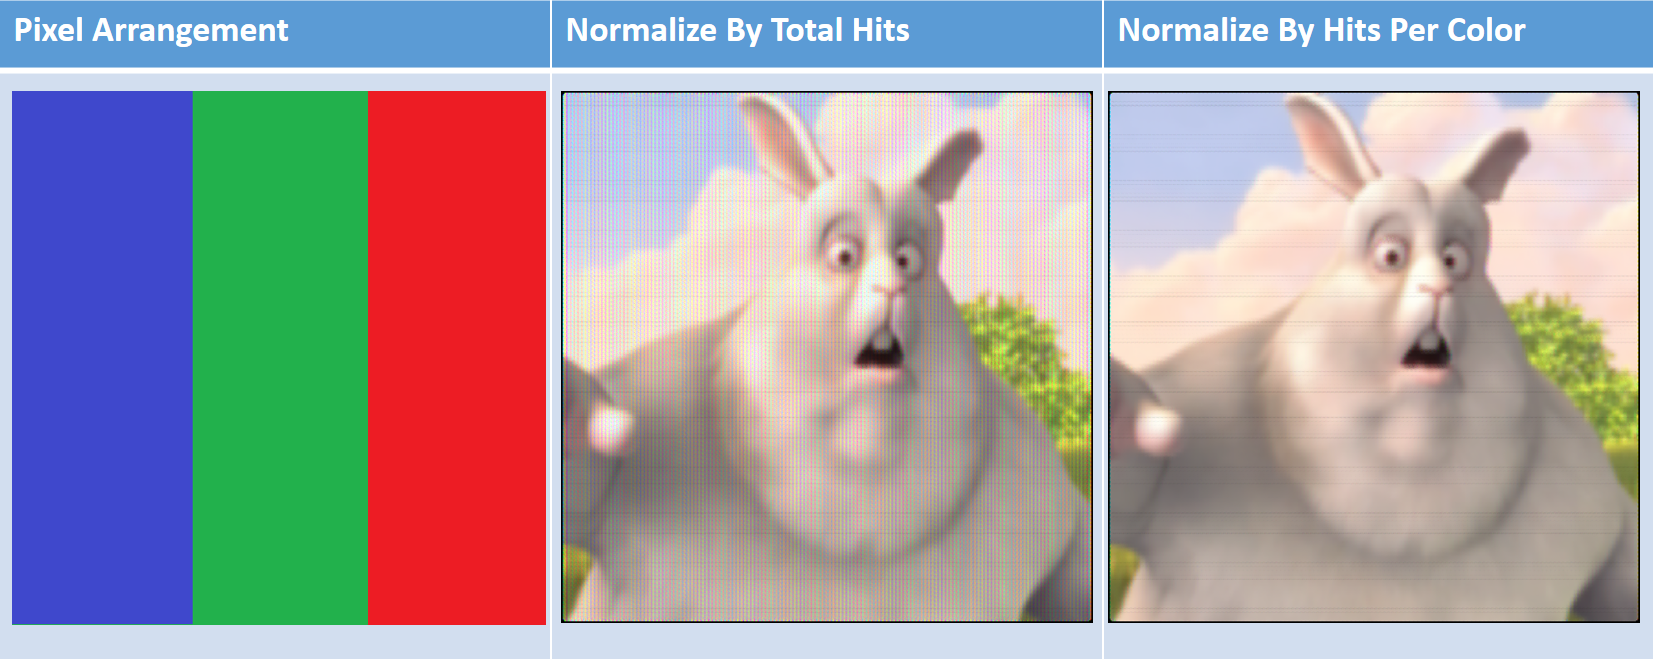
\includegraphics[width=6in]{chapters/chapter7/images/No_Pixel_Arrangement.png}
\end{figure}

\begin{figure}
    \centering
    \textbf{Base Case: RGB Bar}\par\medskip
    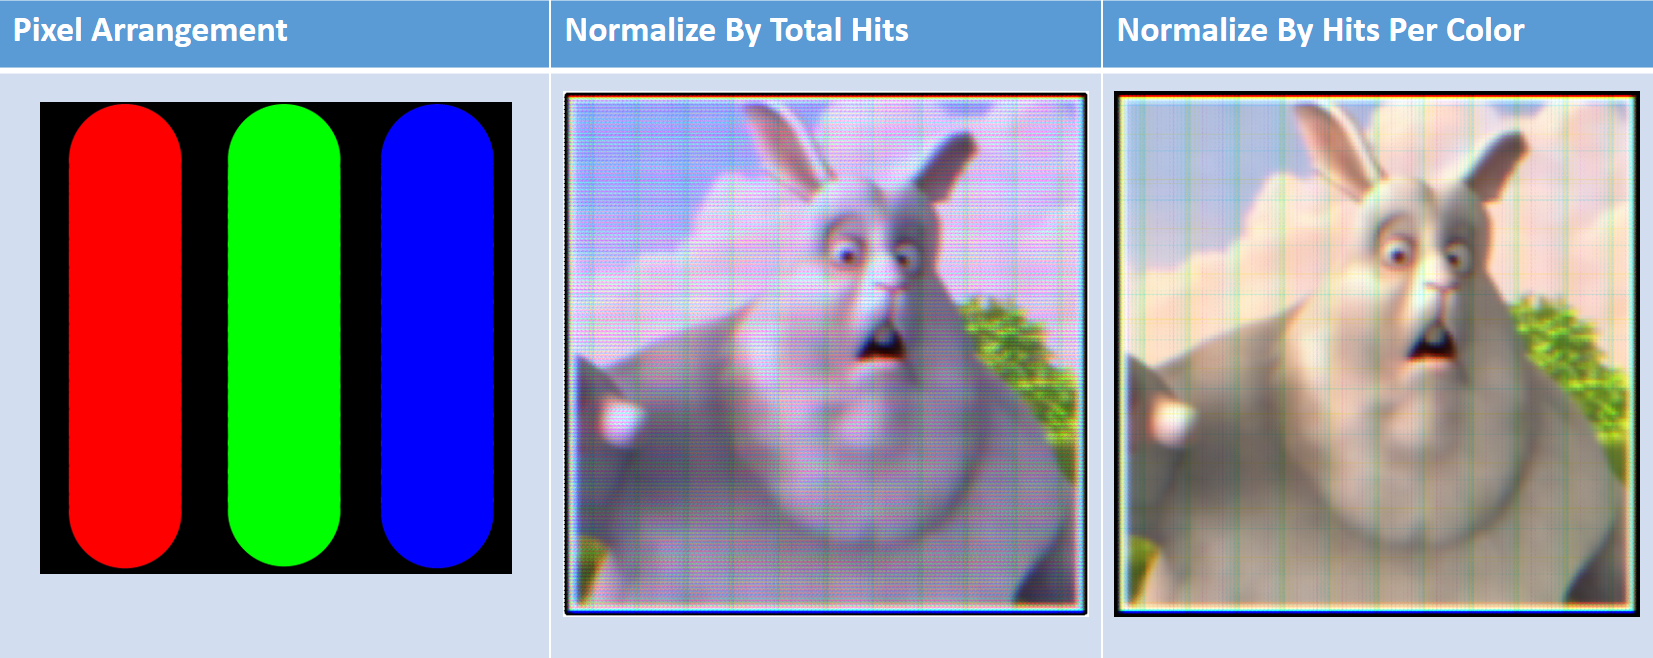
\includegraphics[width=6in]{chapters/chapter7/images/RGB_Bar.png}
\end{figure}

\begin{figure}
    \centering
    \textbf{iPhone}\par\medskip
    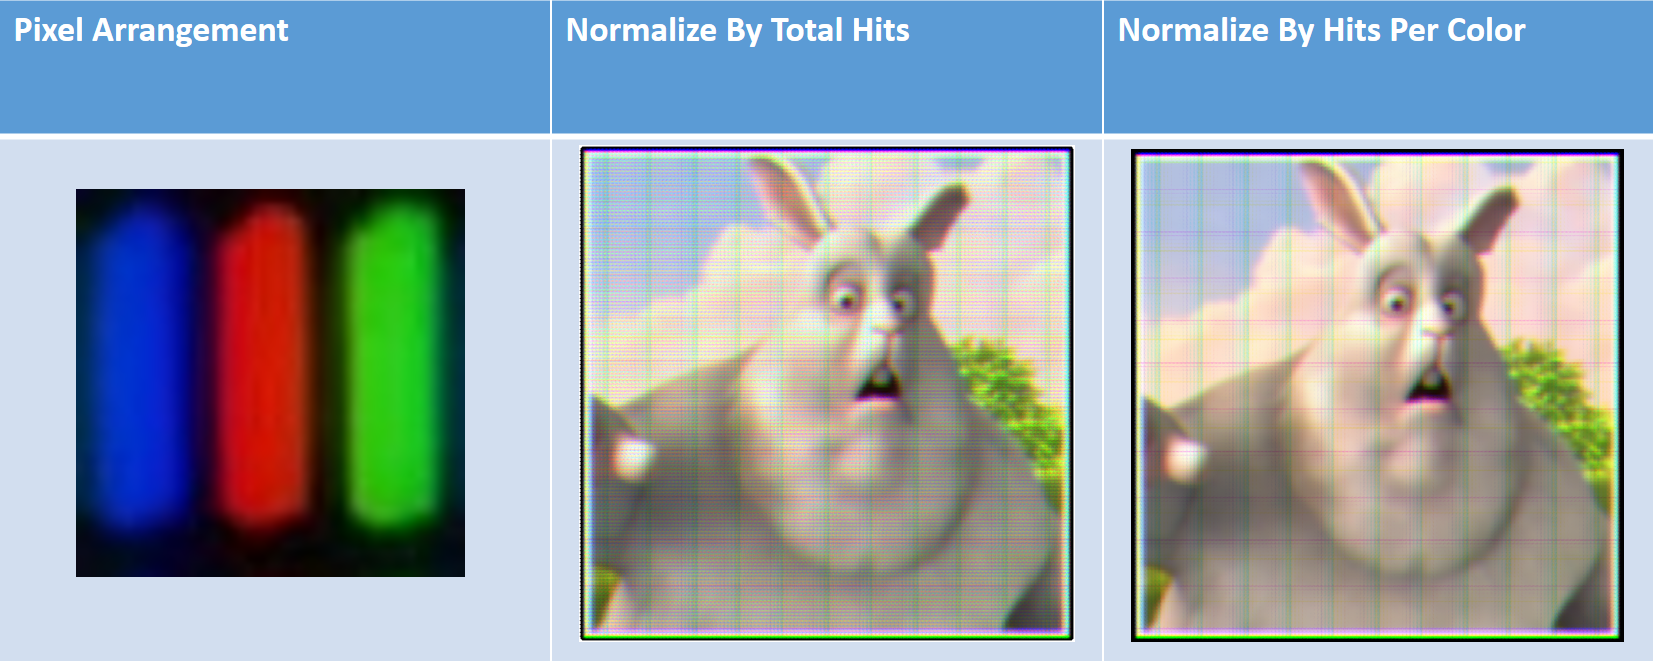
\includegraphics[width=6in]{chapters/chapter7/images/iPhone.png}
\end{figure}

\begin{figure}
    \centering
    \textbf{Samsung Galaxy S2}\par\medskip
    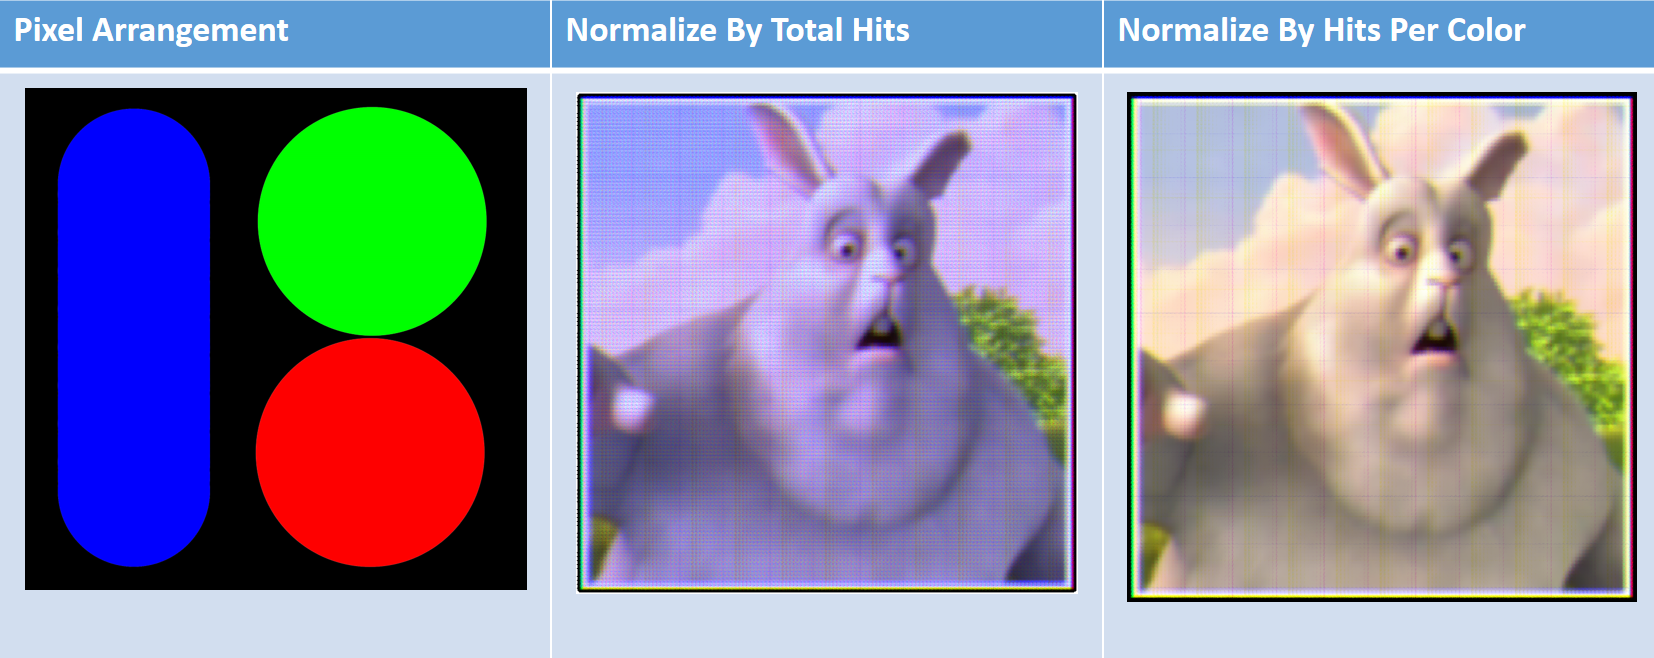
\includegraphics[width=6in]{chapters/chapter7/images/Samsung_Galaxy_S2.png}
\end{figure}

\begin{figure}
    \centering
    \textbf{Samsung Galaxy S3}\par\medskip
    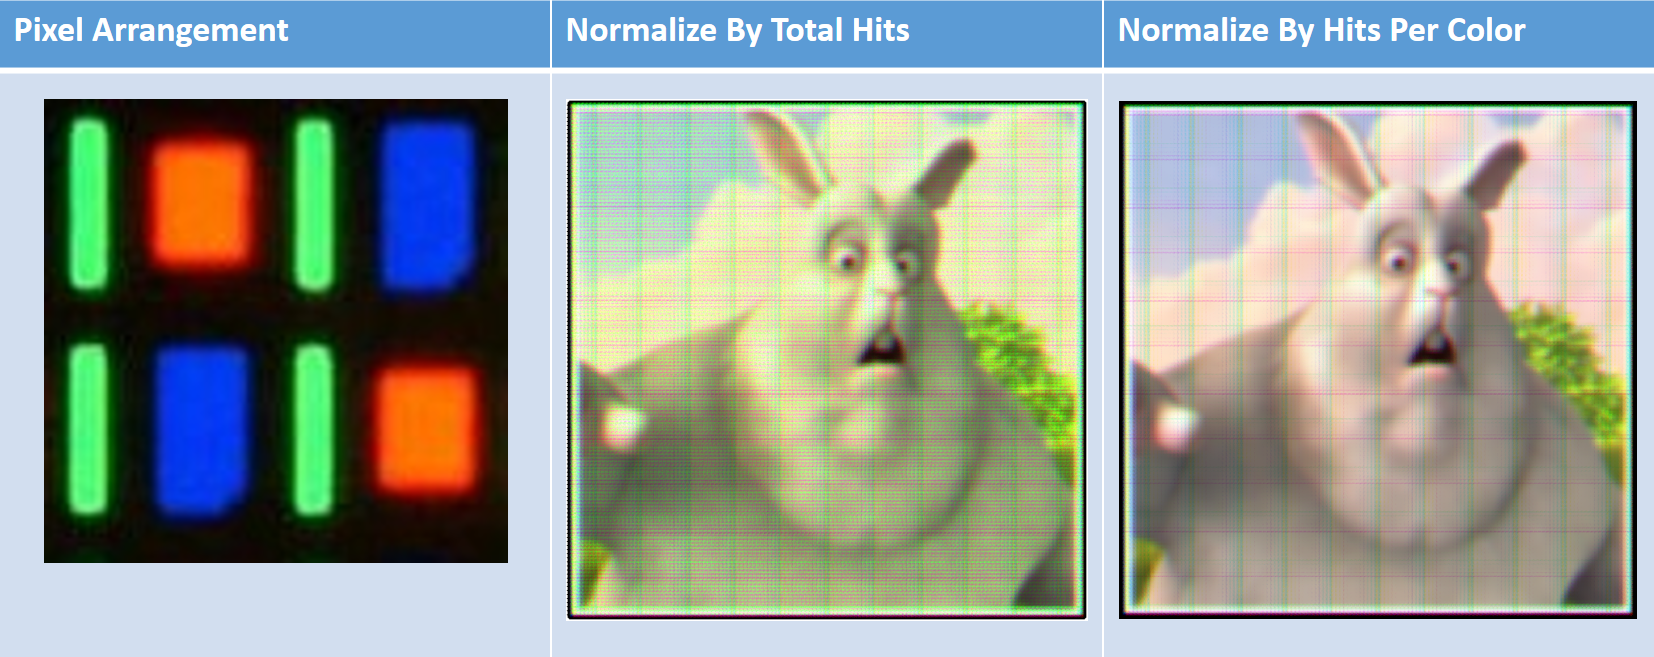
\includegraphics[width=6in]{chapters/chapter7/images/Samsung_Galaxy_S3.png}
\end{figure}

\begin{figure}
    \centering
    \textbf{Samsung Galaxy S4}\par\medskip
    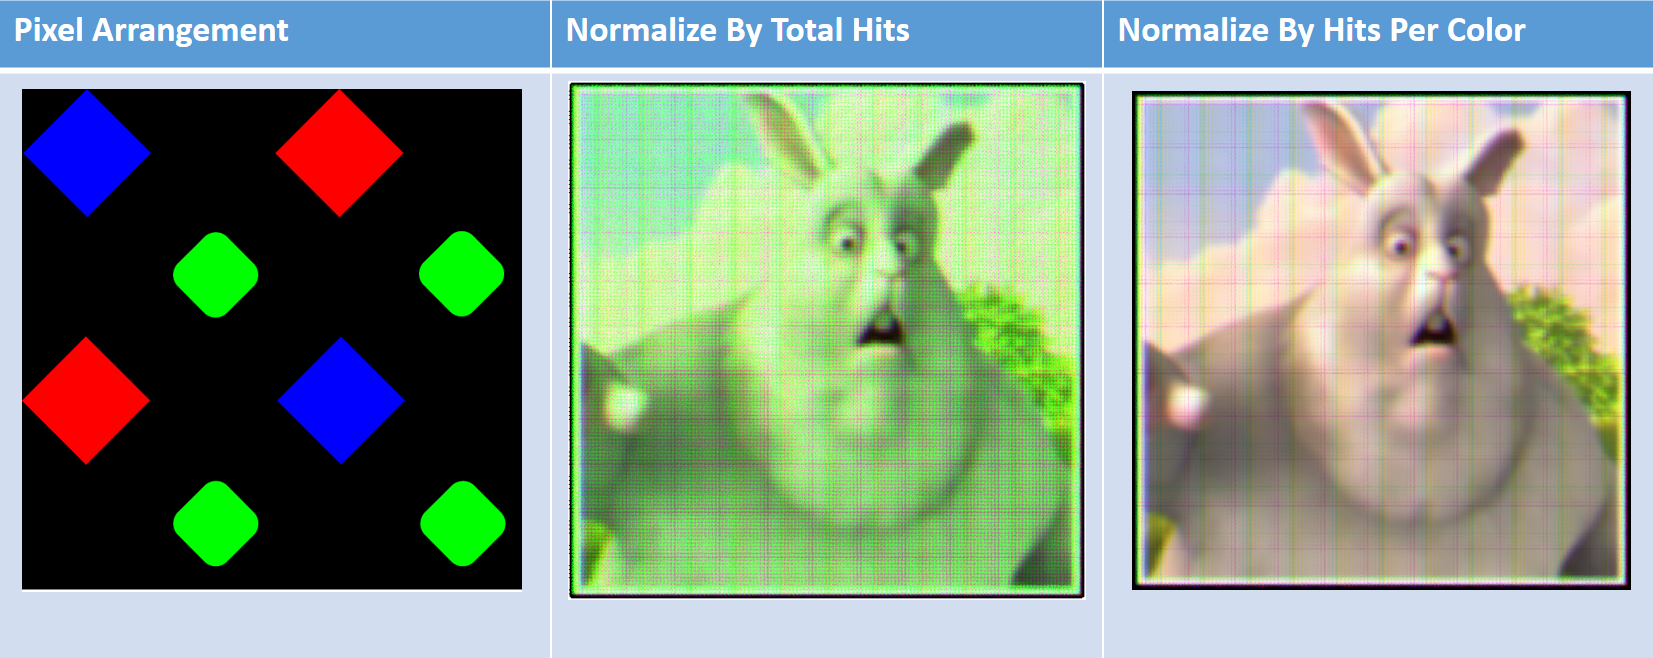
\includegraphics[width=6in]{chapters/chapter7/images/Samsung_Galaxy_S4.png}
\end{figure}

\newpage
\section{Analysis}

% Turn this into a paragraph
Here are few quick observations:
\begin{enumerate}
\item The default simulation (OpenCV RGB bars) yields the best results.

\item The RGB Bar and the Samsung Galaxy S2 have images that are bright when normalized by the total number of hits. 

\item The Samsung Galaxy S3 and especially the Samsung Galaxy S4 have a green shade when normalized by the total number of hits, possibly due to a disproportionate amount of green rays.

\item All images look very clear when normalized by hits per color and yield a similar grid pattern.
\end{enumerate}

As expected, the pixel arrangement creates a large different when you normalize by the total hits because there is a disproportionate amount of red, green, and blue hits when the red, green, and blue components are not equal in area or on different positions of the pixel. However, when I normalize by hits per color, this issue is resolved. The grided pattern may be a result of some pixels on the sensor that have rays traced to unexpected areas on the screen, but it does not interfere much with clear recognition of the bunny.